% SOURCE: edit-harness/results/frame_a/cells/cell_*_real_MIX_C_*.json
% !TEX encoding = UTF-8 Unicode
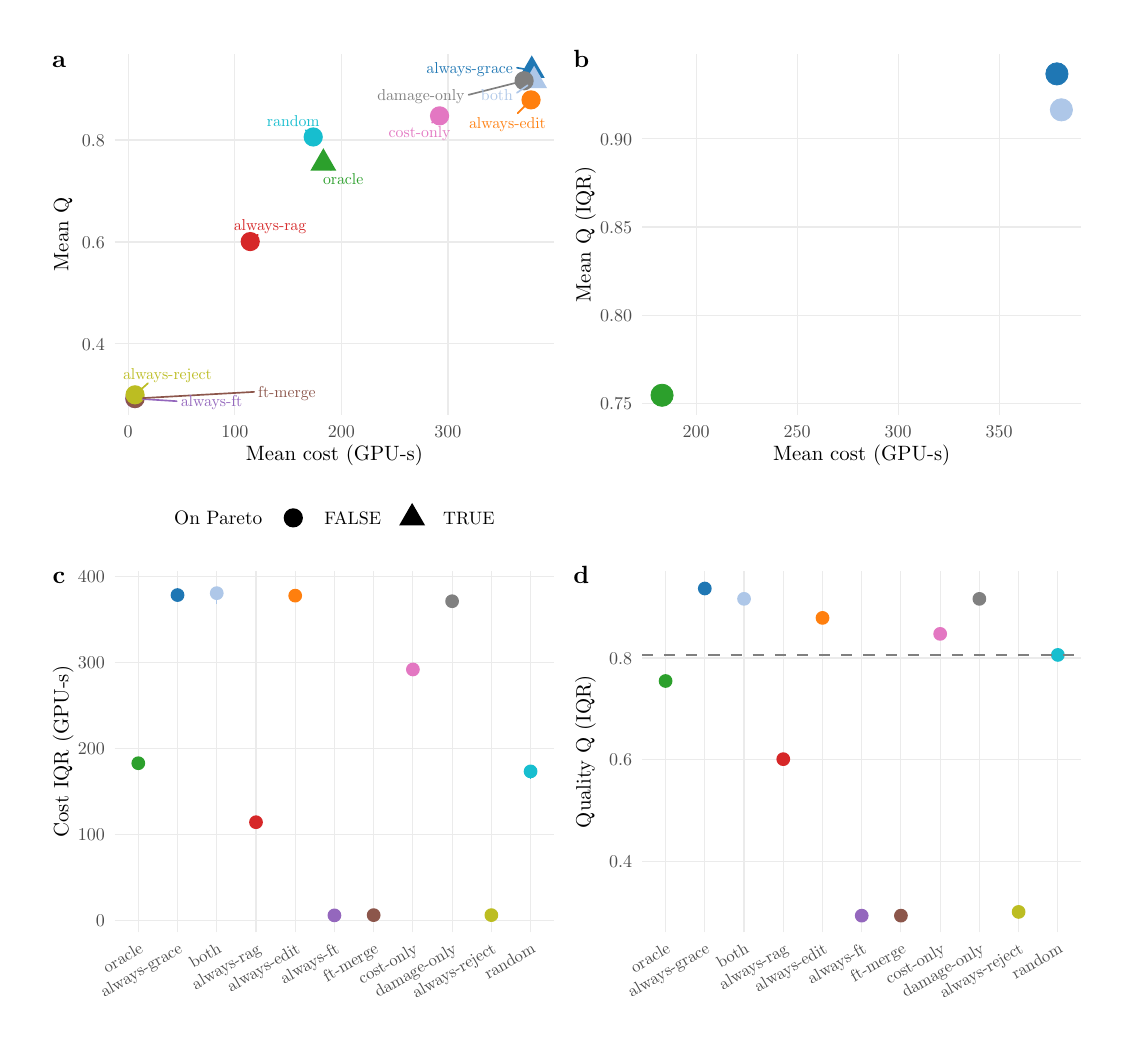
\begin{tikzpicture}[x=1pt,y=1pt]
\definecolor{fillColor}{RGB}{255,255,255}
\path[use as bounding box,fill=fillColor,fill opacity=0.00] (0,0) rectangle (390.26,361.35);
\begin{scope}
\path[clip] (  0.00,  0.00) rectangle (390.26,361.35);
\definecolor{drawColor}{RGB}{255,255,255}
\definecolor{fillColor}{RGB}{255,255,255}

\path[draw=drawColor,line width= 0.6pt,line join=round,line cap=round,fill=fillColor] (  0.00,  0.00) rectangle (390.26,361.35);
\end{scope}
\begin{scope}
\path[clip] (  5.50,168.99) rectangle (194.23,355.85);
\definecolor{fillColor}{RGB}{255,255,255}

\path[fill=fillColor] (  5.50,168.99) rectangle (194.23,355.85);
\end{scope}
\begin{scope}
\path[clip] (194.23,168.99) rectangle (384.76,355.85);
\definecolor{fillColor}{RGB}{255,255,255}

\path[fill=fillColor] (194.23,168.99) rectangle (384.76,355.85);
\end{scope}
\begin{scope}
\path[clip] (  5.50,  5.50) rectangle (194.23,168.99);
\definecolor{fillColor}{RGB}{255,255,255}

\path[fill=fillColor] (  5.50,  5.50) rectangle (194.23,168.99);
\end{scope}
\begin{scope}
\path[clip] (194.23,  5.50) rectangle (384.76,168.99);
\definecolor{fillColor}{RGB}{255,255,255}

\path[fill=fillColor] (194.23,  5.50) rectangle (384.76,168.99);
\end{scope}
\begin{scope}
\path[clip] ( 31.47,221.41) rectangle (190.23,351.85);
\definecolor{drawColor}{gray}{0.92}

\path[draw=drawColor,line width= 0.4pt,line join=round] ( 31.47,247.09) --
	(190.23,247.09);

\path[draw=drawColor,line width= 0.4pt,line join=round] ( 31.47,283.91) --
	(190.23,283.91);

\path[draw=drawColor,line width= 0.4pt,line join=round] ( 31.47,320.74) --
	(190.23,320.74);

\path[draw=drawColor,line width= 0.4pt,line join=round] ( 36.33,221.41) --
	( 36.33,351.85);

\path[draw=drawColor,line width= 0.4pt,line join=round] ( 74.85,221.41) --
	( 74.85,351.85);

\path[draw=drawColor,line width= 0.4pt,line join=round] (113.36,221.41) --
	(113.36,351.85);

\path[draw=drawColor,line width= 0.4pt,line join=round] (151.88,221.41) --
	(151.88,351.85);
\definecolor{fillColor}{RGB}{44,160,44}

\path[fill=fillColor] (106.85,317.79) --
	(111.52,309.69) --
	(102.17,309.69) --
	cycle;
\definecolor{fillColor}{RGB}{31,119,180}

\path[fill=fillColor] (182.15,351.32) --
	(186.83,343.22) --
	(177.48,343.22) --
	cycle;
\definecolor{fillColor}{RGB}{174,199,232}

\path[fill=fillColor] (183.01,347.57) --
	(187.69,339.47) --
	(178.33,339.47) --
	cycle;
\definecolor{fillColor}{RGB}{214,39,40}

\path[fill=fillColor] ( 80.42,284.06) circle (  3.47);
\definecolor{fillColor}{RGB}{255,127,14}

\path[fill=fillColor] (181.89,335.26) circle (  3.47);
\definecolor{fillColor}{RGB}{148,103,189}

\path[fill=fillColor] ( 38.69,227.33) circle (  3.47);
\definecolor{fillColor}{RGB}{140,86,75}

\path[fill=fillColor] ( 38.80,227.33) circle (  3.47);
\definecolor{fillColor}{RGB}{227,119,194}

\path[fill=fillColor] (148.83,329.48) circle (  3.47);
\definecolor{fillColor}{gray}{0.50}

\path[fill=fillColor] (179.39,342.17) circle (  3.47);
\definecolor{fillColor}{RGB}{188,189,34}

\path[fill=fillColor] ( 38.80,228.68) circle (  3.47);
\definecolor{fillColor}{RGB}{23,190,207}

\path[fill=fillColor] (103.18,321.85) circle (  3.47);
\definecolor{drawColor}{RGB}{44,160,44}

\path[draw=drawColor,line width= 0.6pt,line join=round,line cap=round] (109.58,309.96) -- (109.00,310.48);
\definecolor{drawColor}{RGB}{31,119,180}

\path[draw=drawColor,line width= 0.6pt,line join=round,line cap=round] (176.81,346.86) -- (179.32,346.42);
\definecolor{drawColor}{RGB}{174,199,232}

\path[draw=drawColor,line width= 0.6pt,line join=round,line cap=round] (176.79,337.81) -- (180.66,340.52);
\definecolor{drawColor}{RGB}{214,39,40}

\path[draw=drawColor,line width= 0.6pt,line join=round,line cap=round] ( 83.16,286.50) -- ( 82.57,285.97);
\definecolor{drawColor}{RGB}{255,127,14}

\path[draw=drawColor,line width= 0.6pt,line join=round,line cap=round] (177.05,330.43) -- (179.85,333.23);
\definecolor{drawColor}{RGB}{148,103,189}

\path[draw=drawColor,line width= 0.6pt,line join=round,line cap=round] ( 53.86,226.38) -- ( 41.56,227.15);
\definecolor{drawColor}{RGB}{140,86,75}

\path[draw=drawColor,line width= 0.6pt,line join=round,line cap=round] ( 81.83,229.74) -- ( 41.67,227.50);
\definecolor{drawColor}{RGB}{227,119,194}

\path[draw=drawColor,line width= 0.6pt,line join=round,line cap=round] (146.07,327.02) -- (146.68,327.57);
\definecolor{drawColor}{gray}{0.50}

\path[draw=drawColor,line width= 0.6pt,line join=round,line cap=round] (159.32,337.08) -- (176.60,341.46);
\definecolor{drawColor}{RGB}{188,189,34}

\path[draw=drawColor,line width= 0.6pt,line join=round,line cap=round] ( 43.45,232.85) -- ( 40.94,230.60);
\definecolor{drawColor}{RGB}{23,190,207}

\path[draw=drawColor,line width= 0.6pt,line join=round,line cap=round] (100.43,324.29) -- (101.03,323.76);
\definecolor{drawColor}{RGB}{44,160,44}

\node[text=drawColor,anchor=base,inner sep=0pt, outer sep=0pt, scale=  0.57] at (114.01,304.53) {oracle};
\definecolor{drawColor}{RGB}{31,119,180}

\node[text=drawColor,anchor=base,inner sep=0pt, outer sep=0pt, scale=  0.57] at (159.72,344.92) {always-grace};
\definecolor{drawColor}{RGB}{174,199,232}

\node[text=drawColor,anchor=base,inner sep=0pt, outer sep=0pt, scale=  0.57] at (169.52,334.94) {both};
\definecolor{drawColor}{RGB}{214,39,40}

\node[text=drawColor,anchor=base,inner sep=0pt, outer sep=0pt, scale=  0.57] at ( 87.58,288.01) {always-rag};
\definecolor{drawColor}{RGB}{255,127,14}

\node[text=drawColor,anchor=base,inner sep=0pt, outer sep=0pt, scale=  0.57] at (173.37,325.00) {always-edit};
\definecolor{drawColor}{RGB}{148,103,189}

\node[text=drawColor,anchor=base,inner sep=0pt, outer sep=0pt, scale=  0.57] at ( 66.45,224.42) {always-ft};
\definecolor{drawColor}{RGB}{140,86,75}

\node[text=drawColor,anchor=base,inner sep=0pt, outer sep=0pt, scale=  0.57] at ( 93.69,227.78) {ft-merge};
\definecolor{drawColor}{RGB}{227,119,194}

\node[text=drawColor,anchor=base,inner sep=0pt, outer sep=0pt, scale=  0.57] at (141.62,321.60) {cost-only};
\definecolor{drawColor}{gray}{0.50}

\node[text=drawColor,anchor=base,inner sep=0pt, outer sep=0pt, scale=  0.57] at (142.09,334.97) {damage-only};
\definecolor{drawColor}{RGB}{188,189,34}

\node[text=drawColor,anchor=base,inner sep=0pt, outer sep=0pt, scale=  0.57] at ( 50.47,234.36) {always-reject};
\definecolor{drawColor}{RGB}{23,190,207}

\node[text=drawColor,anchor=base,inner sep=0pt, outer sep=0pt, scale=  0.57] at ( 95.98,325.80) {random};
\end{scope}
\begin{scope}
\path[clip] (  0.00,  0.00) rectangle (390.26,361.35);
\definecolor{drawColor}{gray}{0.30}

\node[text=drawColor,anchor=base east,inner sep=0pt, outer sep=0pt, scale=  0.65] at ( 27.87,244.86) {0.4};

\node[text=drawColor,anchor=base east,inner sep=0pt, outer sep=0pt, scale=  0.65] at ( 27.87,281.68) {0.6};

\node[text=drawColor,anchor=base east,inner sep=0pt, outer sep=0pt, scale=  0.65] at ( 27.87,318.50) {0.8};
\end{scope}
\begin{scope}
\path[clip] (  0.00,  0.00) rectangle (390.26,361.35);
\definecolor{drawColor}{gray}{0.30}

\node[text=drawColor,anchor=base,inner sep=0pt, outer sep=0pt, scale=  0.65] at ( 36.33,213.33) {0};

\node[text=drawColor,anchor=base,inner sep=0pt, outer sep=0pt, scale=  0.65] at ( 74.85,213.33) {100};

\node[text=drawColor,anchor=base,inner sep=0pt, outer sep=0pt, scale=  0.65] at (113.36,213.33) {200};

\node[text=drawColor,anchor=base,inner sep=0pt, outer sep=0pt, scale=  0.65] at (151.88,213.33) {300};
\end{scope}
\begin{scope}
\path[clip] (  0.00,  0.00) rectangle (390.26,361.35);
\definecolor{drawColor}{RGB}{0,0,0}

\node[text=drawColor,anchor=base,inner sep=0pt, outer sep=0pt, scale=  0.75] at (110.85,204.90) {Mean cost (GPU-s)};
\end{scope}
\begin{scope}
\path[clip] (  0.00,  0.00) rectangle (390.26,361.35);
\definecolor{drawColor}{RGB}{0,0,0}

\node[text=drawColor,rotate= 90.00,anchor=base,inner sep=0pt, outer sep=0pt, scale=  0.75] at ( 14.67,286.63) {Mean Q};
\end{scope}
\begin{scope}
\path[clip] (  0.00,  0.00) rectangle (390.26,361.35);
\definecolor{drawColor}{RGB}{0,0,0}

\node[text=drawColor,anchor=base west,inner sep=0pt, outer sep=0pt, scale=  0.70] at ( 52.95,181.80) {On Pareto};
\end{scope}
\begin{scope}
\path[clip] (  0.00,  0.00) rectangle (390.26,361.35);
\definecolor{fillColor}{RGB}{0,0,0}

\path[fill=fillColor] ( 95.98,184.21) circle (  3.47);
\end{scope}
\begin{scope}
\path[clip] (  0.00,  0.00) rectangle (390.26,361.35);
\definecolor{fillColor}{RGB}{0,0,0}

\path[fill=fillColor] (138.92,189.61) --
	(143.60,181.52) --
	(134.25,181.52) --
	cycle;
\end{scope}
\begin{scope}
\path[clip] (  0.00,  0.00) rectangle (390.26,361.35);
\definecolor{drawColor}{RGB}{0,0,0}

\node[text=drawColor,anchor=base west,inner sep=0pt, outer sep=0pt, scale=  0.65] at (107.21,181.98) {FALSE};
\end{scope}
\begin{scope}
\path[clip] (  0.00,  0.00) rectangle (390.26,361.35);
\definecolor{drawColor}{RGB}{0,0,0}

\node[text=drawColor,anchor=base west,inner sep=0pt, outer sep=0pt, scale=  0.65] at (150.15,181.98) {TRUE};
\end{scope}
\begin{scope}
\path[clip] (  0.00,  0.00) rectangle (390.26,361.35);
\definecolor{drawColor}{RGB}{0,0,0}

\node[text=drawColor,anchor=base,inner sep=0pt, outer sep=0pt, scale=  0.90] at ( 11.31,346.96) {\bfseries a};
\end{scope}
\begin{scope}
\path[clip] (222.00,221.41) rectangle (380.76,351.85);
\definecolor{drawColor}{gray}{0.92}

\path[draw=drawColor,line width= 0.4pt,line join=round] (222.00,225.55) --
	(380.76,225.55);

\path[draw=drawColor,line width= 0.4pt,line join=round] (222.00,257.43) --
	(380.76,257.43);

\path[draw=drawColor,line width= 0.4pt,line join=round] (222.00,289.31) --
	(380.76,289.31);

\path[draw=drawColor,line width= 0.4pt,line join=round] (222.00,321.18) --
	(380.76,321.18);

\path[draw=drawColor,line width= 0.4pt,line join=round] (241.58,221.41) --
	(241.58,351.85);

\path[draw=drawColor,line width= 0.4pt,line join=round] (278.06,221.41) --
	(278.06,351.85);

\path[draw=drawColor,line width= 0.4pt,line join=round] (314.55,221.41) --
	(314.55,351.85);

\path[draw=drawColor,line width= 0.4pt,line join=round] (351.03,221.41) --
	(351.03,351.85);
\definecolor{drawColor}{RGB}{44,160,44}
\definecolor{fillColor}{RGB}{44,160,44}

\path[draw=drawColor,line width= 0.3pt,line join=round,line cap=round,fill=fillColor] (229.23,228.52) circle (  4.01);
\definecolor{drawColor}{RGB}{31,119,180}
\definecolor{fillColor}{RGB}{31,119,180}

\path[draw=drawColor,line width= 0.3pt,line join=round,line cap=round,fill=fillColor] (371.91,344.65) circle (  4.01);
\definecolor{drawColor}{RGB}{174,199,232}
\definecolor{fillColor}{RGB}{174,199,232}

\path[draw=drawColor,line width= 0.3pt,line join=round,line cap=round,fill=fillColor] (373.53,331.66) circle (  4.01);
\definecolor{drawColor}{RGB}{44,160,44}

\path[draw=drawColor,line width= 0.5pt,line join=round] (229.22,230.39) --
	(229.25,230.39);

\path[draw=drawColor,line width= 0.5pt,line join=round] (229.23,230.39) --
	(229.23,227.33);

\path[draw=drawColor,line width= 0.5pt,line join=round] (229.22,227.33) --
	(229.25,227.33);
\definecolor{drawColor}{RGB}{31,119,180}

\path[draw=drawColor,line width= 0.5pt,line join=round] (371.89,345.92) --
	(371.92,345.92);

\path[draw=drawColor,line width= 0.5pt,line join=round] (371.91,345.92) --
	(371.91,343.63);

\path[draw=drawColor,line width= 0.5pt,line join=round] (371.89,343.63) --
	(371.92,343.63);
\definecolor{drawColor}{RGB}{174,199,232}

\path[draw=drawColor,line width= 0.5pt,line join=round] (373.51,332.01) --
	(373.54,332.01);

\path[draw=drawColor,line width= 0.5pt,line join=round] (373.53,332.01) --
	(373.53,330.99);

\path[draw=drawColor,line width= 0.5pt,line join=round] (373.51,330.99) --
	(373.54,330.99);
\end{scope}
\begin{scope}
\path[clip] (  0.00,  0.00) rectangle (390.26,361.35);
\definecolor{drawColor}{gray}{0.30}

\node[text=drawColor,anchor=base east,inner sep=0pt, outer sep=0pt, scale=  0.65] at (218.40,223.31) {0.75};

\node[text=drawColor,anchor=base east,inner sep=0pt, outer sep=0pt, scale=  0.65] at (218.40,255.19) {0.80};

\node[text=drawColor,anchor=base east,inner sep=0pt, outer sep=0pt, scale=  0.65] at (218.40,287.07) {0.85};

\node[text=drawColor,anchor=base east,inner sep=0pt, outer sep=0pt, scale=  0.65] at (218.40,318.95) {0.90};
\end{scope}
\begin{scope}
\path[clip] (  0.00,  0.00) rectangle (390.26,361.35);
\definecolor{drawColor}{gray}{0.30}

\node[text=drawColor,anchor=base,inner sep=0pt, outer sep=0pt, scale=  0.65] at (241.58,213.33) {200};

\node[text=drawColor,anchor=base,inner sep=0pt, outer sep=0pt, scale=  0.65] at (278.06,213.33) {250};

\node[text=drawColor,anchor=base,inner sep=0pt, outer sep=0pt, scale=  0.65] at (314.55,213.33) {300};

\node[text=drawColor,anchor=base,inner sep=0pt, outer sep=0pt, scale=  0.65] at (351.03,213.33) {350};
\end{scope}
\begin{scope}
\path[clip] (  0.00,  0.00) rectangle (390.26,361.35);
\definecolor{drawColor}{RGB}{0,0,0}

\node[text=drawColor,anchor=base,inner sep=0pt, outer sep=0pt, scale=  0.75] at (301.38,204.90) {Mean cost (GPU-s)};
\end{scope}
\begin{scope}
\path[clip] (  0.00,  0.00) rectangle (390.26,361.35);
\definecolor{drawColor}{RGB}{0,0,0}

\node[text=drawColor,rotate= 90.00,anchor=base,inner sep=0pt, outer sep=0pt, scale=  0.75] at (203.39,286.63) {Mean Q (IQR)};
\end{scope}
\begin{scope}
\path[clip] (  0.00,  0.00) rectangle (390.26,361.35);
\definecolor{drawColor}{RGB}{0,0,0}

\node[text=drawColor,anchor=base,inner sep=0pt, outer sep=0pt, scale=  0.90] at (200.05,346.96) {\bfseries b};
\end{scope}
\begin{scope}
\path[clip] ( 31.47, 34.54) rectangle (190.23,164.99);
\definecolor{drawColor}{gray}{0.92}

\path[draw=drawColor,line width= 0.4pt,line join=round] ( 31.47, 38.68) --
	(190.23, 38.68);

\path[draw=drawColor,line width= 0.4pt,line join=round] ( 31.47, 69.75) --
	(190.23, 69.75);

\path[draw=drawColor,line width= 0.4pt,line join=round] ( 31.47,100.82) --
	(190.23,100.82);

\path[draw=drawColor,line width= 0.4pt,line join=round] ( 31.47,131.90) --
	(190.23,131.90);

\path[draw=drawColor,line width= 0.4pt,line join=round] ( 31.47,162.97) --
	(190.23,162.97);

\path[draw=drawColor,line width= 0.4pt,line join=round] ( 39.98, 34.54) --
	( 39.98,164.99);

\path[draw=drawColor,line width= 0.4pt,line join=round] ( 54.15, 34.54) --
	( 54.15,164.99);

\path[draw=drawColor,line width= 0.4pt,line join=round] ( 68.32, 34.54) --
	( 68.32,164.99);

\path[draw=drawColor,line width= 0.4pt,line join=round] ( 82.50, 34.54) --
	( 82.50,164.99);

\path[draw=drawColor,line width= 0.4pt,line join=round] ( 96.67, 34.54) --
	( 96.67,164.99);

\path[draw=drawColor,line width= 0.4pt,line join=round] (110.85, 34.54) --
	(110.85,164.99);

\path[draw=drawColor,line width= 0.4pt,line join=round] (125.02, 34.54) --
	(125.02,164.99);

\path[draw=drawColor,line width= 0.4pt,line join=round] (139.20, 34.54) --
	(139.20,164.99);

\path[draw=drawColor,line width= 0.4pt,line join=round] (153.37, 34.54) --
	(153.37,164.99);

\path[draw=drawColor,line width= 0.4pt,line join=round] (167.55, 34.54) --
	(167.55,164.99);

\path[draw=drawColor,line width= 0.4pt,line join=round] (181.72, 34.54) --
	(181.72,164.99);
\definecolor{drawColor}{RGB}{44,160,44}

\path[draw=drawColor,line width= 0.4pt,line join=round] ( 39.98, 94.85) -- ( 39.98, 96.20);
\definecolor{drawColor}{RGB}{31,119,180}

\path[draw=drawColor,line width= 0.4pt,line join=round] ( 54.15,154.20) -- ( 54.15,157.86);
\definecolor{drawColor}{RGB}{174,199,232}

\path[draw=drawColor,line width= 0.4pt,line join=round] ( 68.32,153.03) -- ( 68.32,159.06);
\definecolor{drawColor}{RGB}{214,39,40}

\path[draw=drawColor,line width= 0.4pt,line join=round] ( 82.50, 73.68) -- ( 82.50, 74.75);
\definecolor{drawColor}{RGB}{255,127,14}

\path[draw=drawColor,line width= 0.4pt,line join=round] ( 96.67,155.91) -- ( 96.67,156.37);
\definecolor{drawColor}{RGB}{148,103,189}

\path[draw=drawColor,line width= 0.4pt,line join=round] (110.85, 40.47) -- (110.85, 40.64);
\definecolor{drawColor}{RGB}{140,86,75}

\path[draw=drawColor,line width= 0.4pt,line join=round] (125.02, 40.51) -- (125.02, 40.75);
\definecolor{drawColor}{RGB}{227,119,194}

\path[draw=drawColor,line width= 0.4pt,line join=round] (139.20,127.07) -- (139.20,130.68);
\definecolor{drawColor}{gray}{0.50}

\path[draw=drawColor,line width= 0.4pt,line join=round] (153.37,153.59) -- (153.37,154.44);
\definecolor{drawColor}{RGB}{188,189,34}

\path[draw=drawColor,line width= 0.4pt,line join=round] (167.55, 40.50) -- (167.55, 40.77);
\definecolor{drawColor}{RGB}{23,190,207}

\path[draw=drawColor,line width= 0.4pt,line join=round] (181.72, 89.93) -- (181.72, 94.49);
\definecolor{drawColor}{RGB}{44,160,44}
\definecolor{fillColor}{RGB}{44,160,44}

\path[draw=drawColor,line width= 0.5pt,line join=round,line cap=round,fill=fillColor] ( 39.98, 95.56) circle (  2.23);
\definecolor{drawColor}{RGB}{31,119,180}
\definecolor{fillColor}{RGB}{31,119,180}

\path[draw=drawColor,line width= 0.5pt,line join=round,line cap=round,fill=fillColor] ( 54.15,156.32) circle (  2.23);
\definecolor{drawColor}{RGB}{174,199,232}
\definecolor{fillColor}{RGB}{174,199,232}

\path[draw=drawColor,line width= 0.5pt,line join=round,line cap=round,fill=fillColor] ( 68.32,157.01) circle (  2.23);
\definecolor{drawColor}{RGB}{214,39,40}
\definecolor{fillColor}{RGB}{214,39,40}

\path[draw=drawColor,line width= 0.5pt,line join=round,line cap=round,fill=fillColor] ( 82.50, 74.24) circle (  2.23);
\definecolor{drawColor}{RGB}{255,127,14}
\definecolor{fillColor}{RGB}{255,127,14}

\path[draw=drawColor,line width= 0.5pt,line join=round,line cap=round,fill=fillColor] ( 96.67,156.11) circle (  2.23);
\definecolor{drawColor}{RGB}{148,103,189}
\definecolor{fillColor}{RGB}{148,103,189}

\path[draw=drawColor,line width= 0.5pt,line join=round,line cap=round,fill=fillColor] (110.85, 40.58) circle (  2.23);
\definecolor{drawColor}{RGB}{140,86,75}
\definecolor{fillColor}{RGB}{140,86,75}

\path[draw=drawColor,line width= 0.5pt,line join=round,line cap=round,fill=fillColor] (125.02, 40.67) circle (  2.23);
\definecolor{drawColor}{RGB}{227,119,194}
\definecolor{fillColor}{RGB}{227,119,194}

\path[draw=drawColor,line width= 0.5pt,line join=round,line cap=round,fill=fillColor] (139.20,129.44) circle (  2.23);
\definecolor{drawColor}{gray}{0.50}
\definecolor{fillColor}{gray}{0.50}

\path[draw=drawColor,line width= 0.5pt,line join=round,line cap=round,fill=fillColor] (153.37,154.09) circle (  2.23);
\definecolor{drawColor}{RGB}{188,189,34}
\definecolor{fillColor}{RGB}{188,189,34}

\path[draw=drawColor,line width= 0.5pt,line join=round,line cap=round,fill=fillColor] (167.55, 40.67) circle (  2.23);
\definecolor{drawColor}{RGB}{23,190,207}
\definecolor{fillColor}{RGB}{23,190,207}

\path[draw=drawColor,line width= 0.5pt,line join=round,line cap=round,fill=fillColor] (181.72, 92.60) circle (  2.23);
\end{scope}
\begin{scope}
\path[clip] (  0.00,  0.00) rectangle (390.26,361.35);
\definecolor{drawColor}{gray}{0.30}

\node[text=drawColor,anchor=base east,inner sep=0pt, outer sep=0pt, scale=  0.65] at ( 27.87, 36.44) {0};

\node[text=drawColor,anchor=base east,inner sep=0pt, outer sep=0pt, scale=  0.65] at ( 27.87, 67.51) {100};

\node[text=drawColor,anchor=base east,inner sep=0pt, outer sep=0pt, scale=  0.65] at ( 27.87, 98.58) {200};

\node[text=drawColor,anchor=base east,inner sep=0pt, outer sep=0pt, scale=  0.65] at ( 27.87,129.66) {300};

\node[text=drawColor,anchor=base east,inner sep=0pt, outer sep=0pt, scale=  0.65] at ( 27.87,160.73) {400};
\end{scope}
\begin{scope}
\path[clip] (  0.00,  0.00) rectangle (390.26,361.35);
\definecolor{drawColor}{gray}{0.30}

\node[text=drawColor,rotate= 30.00,anchor=base east,inner sep=0pt, outer sep=0pt, scale=  0.60] at ( 42.04, 27.36) {oracle};

\node[text=drawColor,rotate= 30.00,anchor=base east,inner sep=0pt, outer sep=0pt, scale=  0.60] at ( 56.22, 27.36) {always-grace};

\node[text=drawColor,rotate= 30.00,anchor=base east,inner sep=0pt, outer sep=0pt, scale=  0.60] at ( 70.39, 27.36) {both};

\node[text=drawColor,rotate= 30.00,anchor=base east,inner sep=0pt, outer sep=0pt, scale=  0.60] at ( 84.57, 27.36) {always-rag};

\node[text=drawColor,rotate= 30.00,anchor=base east,inner sep=0pt, outer sep=0pt, scale=  0.60] at ( 98.74, 27.36) {always-edit};

\node[text=drawColor,rotate= 30.00,anchor=base east,inner sep=0pt, outer sep=0pt, scale=  0.60] at (112.91, 27.36) {always-ft};

\node[text=drawColor,rotate= 30.00,anchor=base east,inner sep=0pt, outer sep=0pt, scale=  0.60] at (127.09, 27.36) {ft-merge};

\node[text=drawColor,rotate= 30.00,anchor=base east,inner sep=0pt, outer sep=0pt, scale=  0.60] at (141.26, 27.36) {cost-only};

\node[text=drawColor,rotate= 30.00,anchor=base east,inner sep=0pt, outer sep=0pt, scale=  0.60] at (155.44, 27.36) {damage-only};

\node[text=drawColor,rotate= 30.00,anchor=base east,inner sep=0pt, outer sep=0pt, scale=  0.60] at (169.61, 27.36) {always-reject};

\node[text=drawColor,rotate= 30.00,anchor=base east,inner sep=0pt, outer sep=0pt, scale=  0.60] at (183.79, 27.36) {random};
\end{scope}
\begin{scope}
\path[clip] (  0.00,  0.00) rectangle (390.26,361.35);
\definecolor{drawColor}{RGB}{0,0,0}

\node[text=drawColor,rotate= 90.00,anchor=base,inner sep=0pt, outer sep=0pt, scale=  0.75] at ( 14.67, 99.77) {Cost IQR (GPU-s)};
\end{scope}
\begin{scope}
\path[clip] (  0.00,  0.00) rectangle (390.26,361.35);
\definecolor{drawColor}{RGB}{0,0,0}

\node[text=drawColor,anchor=base,inner sep=0pt, outer sep=0pt, scale=  0.90] at ( 11.31,160.33) {\bfseries c};
\end{scope}
\begin{scope}
\path[clip] (222.00, 34.54) rectangle (380.76,164.99);
\definecolor{drawColor}{gray}{0.92}

\path[draw=drawColor,line width= 0.4pt,line join=round] (222.00, 60.18) --
	(380.76, 60.18);

\path[draw=drawColor,line width= 0.4pt,line join=round] (222.00, 96.88) --
	(380.76, 96.88);

\path[draw=drawColor,line width= 0.4pt,line join=round] (222.00,133.59) --
	(380.76,133.59);

\path[draw=drawColor,line width= 0.4pt,line join=round] (230.51, 34.54) --
	(230.51,164.99);

\path[draw=drawColor,line width= 0.4pt,line join=round] (244.68, 34.54) --
	(244.68,164.99);

\path[draw=drawColor,line width= 0.4pt,line join=round] (258.86, 34.54) --
	(258.86,164.99);

\path[draw=drawColor,line width= 0.4pt,line join=round] (273.03, 34.54) --
	(273.03,164.99);

\path[draw=drawColor,line width= 0.4pt,line join=round] (287.21, 34.54) --
	(287.21,164.99);

\path[draw=drawColor,line width= 0.4pt,line join=round] (301.38, 34.54) --
	(301.38,164.99);

\path[draw=drawColor,line width= 0.4pt,line join=round] (315.55, 34.54) --
	(315.55,164.99);

\path[draw=drawColor,line width= 0.4pt,line join=round] (329.73, 34.54) --
	(329.73,164.99);

\path[draw=drawColor,line width= 0.4pt,line join=round] (343.90, 34.54) --
	(343.90,164.99);

\path[draw=drawColor,line width= 0.4pt,line join=round] (358.08, 34.54) --
	(358.08,164.99);

\path[draw=drawColor,line width= 0.4pt,line join=round] (372.25, 34.54) --
	(372.25,164.99);
\definecolor{drawColor}{RGB}{44,160,44}

\path[draw=drawColor,line width= 0.4pt,line join=round] (230.51,124.92) -- (230.51,125.80);
\definecolor{drawColor}{RGB}{31,119,180}

\path[draw=drawColor,line width= 0.4pt,line join=round] (244.68,158.40) -- (244.68,159.06);
\definecolor{drawColor}{RGB}{174,199,232}

\path[draw=drawColor,line width= 0.4pt,line join=round] (258.86,154.76) -- (258.86,155.06);
\definecolor{drawColor}{RGB}{214,39,40}

\path[draw=drawColor,line width= 0.4pt,line join=round] (273.03, 97.03) -- (273.03, 97.03);
\definecolor{drawColor}{RGB}{255,127,14}

\path[draw=drawColor,line width= 0.4pt,line join=round] (287.21,147.54) -- (287.21,148.34);
\definecolor{drawColor}{RGB}{148,103,189}

\path[draw=drawColor,line width= 0.4pt,line join=round] (301.38, 40.47) -- (301.38, 40.49);
\definecolor{drawColor}{RGB}{140,86,75}

\path[draw=drawColor,line width= 0.4pt,line join=round] (315.55, 40.47) -- (315.55, 40.49);
\definecolor{drawColor}{RGB}{227,119,194}

\path[draw=drawColor,line width= 0.4pt,line join=round] (329.73,140.39) -- (329.73,143.66);
\definecolor{drawColor}{gray}{0.50}

\path[draw=drawColor,line width= 0.4pt,line join=round] (343.90,154.76) -- (343.90,155.06);
\definecolor{drawColor}{RGB}{188,189,34}

\path[draw=drawColor,line width= 0.4pt,line join=round] (358.08, 41.83) -- (358.08, 41.83);
\definecolor{drawColor}{RGB}{23,190,207}

\path[draw=drawColor,line width= 0.4pt,line join=round] (372.25,133.67) -- (372.25,135.45);
\definecolor{drawColor}{RGB}{44,160,44}
\definecolor{fillColor}{RGB}{44,160,44}

\path[draw=drawColor,line width= 0.5pt,line join=round,line cap=round,fill=fillColor] (230.51,125.27) circle (  2.23);
\definecolor{drawColor}{RGB}{31,119,180}
\definecolor{fillColor}{RGB}{31,119,180}

\path[draw=drawColor,line width= 0.5pt,line join=round,line cap=round,fill=fillColor] (244.68,158.69) circle (  2.23);
\definecolor{drawColor}{RGB}{174,199,232}
\definecolor{fillColor}{RGB}{174,199,232}

\path[draw=drawColor,line width= 0.5pt,line join=round,line cap=round,fill=fillColor] (258.86,154.95) circle (  2.23);
\definecolor{drawColor}{RGB}{214,39,40}
\definecolor{fillColor}{RGB}{214,39,40}

\path[draw=drawColor,line width= 0.5pt,line join=round,line cap=round,fill=fillColor] (273.03, 97.03) circle (  2.23);
\definecolor{drawColor}{RGB}{255,127,14}
\definecolor{fillColor}{RGB}{255,127,14}

\path[draw=drawColor,line width= 0.5pt,line join=round,line cap=round,fill=fillColor] (287.21,148.07) circle (  2.23);
\definecolor{drawColor}{RGB}{148,103,189}
\definecolor{fillColor}{RGB}{148,103,189}

\path[draw=drawColor,line width= 0.5pt,line join=round,line cap=round,fill=fillColor] (301.38, 40.48) circle (  2.23);
\definecolor{drawColor}{RGB}{140,86,75}
\definecolor{fillColor}{RGB}{140,86,75}

\path[draw=drawColor,line width= 0.5pt,line join=round,line cap=round,fill=fillColor] (315.55, 40.48) circle (  2.23);
\definecolor{drawColor}{RGB}{227,119,194}
\definecolor{fillColor}{RGB}{227,119,194}

\path[draw=drawColor,line width= 0.5pt,line join=round,line cap=round,fill=fillColor] (329.73,142.30) circle (  2.23);
\definecolor{drawColor}{gray}{0.50}
\definecolor{fillColor}{gray}{0.50}

\path[draw=drawColor,line width= 0.5pt,line join=round,line cap=round,fill=fillColor] (343.90,154.95) circle (  2.23);
\definecolor{drawColor}{RGB}{188,189,34}
\definecolor{fillColor}{RGB}{188,189,34}

\path[draw=drawColor,line width= 0.5pt,line join=round,line cap=round,fill=fillColor] (358.08, 41.83) circle (  2.23);
\definecolor{drawColor}{RGB}{23,190,207}
\definecolor{fillColor}{RGB}{23,190,207}

\path[draw=drawColor,line width= 0.5pt,line join=round,line cap=round,fill=fillColor] (372.25,134.69) circle (  2.23);
\definecolor{drawColor}{gray}{0.50}

\path[draw=drawColor,line width= 0.5pt,dash pattern=on 4pt off 4pt ,line join=round] (222.00,134.69) -- (380.76,134.69);
\end{scope}
\begin{scope}
\path[clip] (  0.00,  0.00) rectangle (390.26,361.35);
\definecolor{drawColor}{gray}{0.30}

\node[text=drawColor,anchor=base east,inner sep=0pt, outer sep=0pt, scale=  0.65] at (218.40, 57.94) {0.4};

\node[text=drawColor,anchor=base east,inner sep=0pt, outer sep=0pt, scale=  0.65] at (218.40, 94.64) {0.6};

\node[text=drawColor,anchor=base east,inner sep=0pt, outer sep=0pt, scale=  0.65] at (218.40,131.35) {0.8};
\end{scope}
\begin{scope}
\path[clip] (  0.00,  0.00) rectangle (390.26,361.35);
\definecolor{drawColor}{gray}{0.30}

\node[text=drawColor,rotate= 30.00,anchor=base east,inner sep=0pt, outer sep=0pt, scale=  0.60] at (232.57, 27.36) {oracle};

\node[text=drawColor,rotate= 30.00,anchor=base east,inner sep=0pt, outer sep=0pt, scale=  0.60] at (246.75, 27.36) {always-grace};

\node[text=drawColor,rotate= 30.00,anchor=base east,inner sep=0pt, outer sep=0pt, scale=  0.60] at (260.92, 27.36) {both};

\node[text=drawColor,rotate= 30.00,anchor=base east,inner sep=0pt, outer sep=0pt, scale=  0.60] at (275.10, 27.36) {always-rag};

\node[text=drawColor,rotate= 30.00,anchor=base east,inner sep=0pt, outer sep=0pt, scale=  0.60] at (289.27, 27.36) {always-edit};

\node[text=drawColor,rotate= 30.00,anchor=base east,inner sep=0pt, outer sep=0pt, scale=  0.60] at (303.45, 27.36) {always-ft};

\node[text=drawColor,rotate= 30.00,anchor=base east,inner sep=0pt, outer sep=0pt, scale=  0.60] at (317.62, 27.36) {ft-merge};

\node[text=drawColor,rotate= 30.00,anchor=base east,inner sep=0pt, outer sep=0pt, scale=  0.60] at (331.80, 27.36) {cost-only};

\node[text=drawColor,rotate= 30.00,anchor=base east,inner sep=0pt, outer sep=0pt, scale=  0.60] at (345.97, 27.36) {damage-only};

\node[text=drawColor,rotate= 30.00,anchor=base east,inner sep=0pt, outer sep=0pt, scale=  0.60] at (360.14, 27.36) {always-reject};

\node[text=drawColor,rotate= 30.00,anchor=base east,inner sep=0pt, outer sep=0pt, scale=  0.60] at (374.32, 27.36) {random};
\end{scope}
\begin{scope}
\path[clip] (  0.00,  0.00) rectangle (390.26,361.35);
\definecolor{drawColor}{RGB}{0,0,0}

\node[text=drawColor,rotate= 90.00,anchor=base,inner sep=0pt, outer sep=0pt, scale=  0.75] at (203.39, 99.77) {Quality Q (IQR)};
\end{scope}
\begin{scope}
\path[clip] (  0.00,  0.00) rectangle (390.26,361.35);
\definecolor{drawColor}{RGB}{0,0,0}

\node[text=drawColor,anchor=base,inner sep=0pt, outer sep=0pt, scale=  0.90] at (200.05,160.33) {\bfseries d};
\end{scope}
\end{tikzpicture}
